
Los resultados de los casos de prueba se encuentran 
organizados en un recurso dividido por carpetas, donde 
se almacenan los archivos de salida de los programas \textbf{bf.cpp},\textbf{dp.cpp} y 
el dataset correspondiente. Estos archivos contienen las cadenas comparadas, 
la distancia calculada, la distancia esperada correcta, un indicador con la correctitud
del resultado, el tiempo de ejecución, y las operaciones que producen 
la distancia mínima de edición junto con sus costos. Además, al final de cada archivo, 
se muestra el tiempo promedio de ejecución del dataset procesado.

Para obtener los resultados a continuación, 
es necesario ejecutar los programas mencionados.
El tiempo fue medido utilizando
la biblioteca \textbf{chrono} de C++. También se considera el tiempo promedio de ejecución 
como medida representativa, salvo que se indique lo contrario.

El uso de memoria RAM se determinó utilizando la herramienta \textbf{Massif} 
de Valgrind, que toma muestras del uso de memoria durante la ejecución del programa 
y genera un gráfico con estas métricas.

Las instrucciones detalladas para la ejecución de los programas se encuentran aquí. 


\begin{enumerate}
    \item Transposiciones con matrices de costo estándar y costo modificado
    
        \begin{table}[H]
        \centering
        \begin{tabular}{|c|c|c|}
        \hline
        \textbf{Tipo/Data} & \textbf{Transposiciones costo estándar} & \textbf{Transposiciones costo modificado}\\ \hline
        Fuerza Bruta (ms) & 188.489 & 193.375\\ \hline
        Programación Dinámica (ms) & 0.0956651 & 0.0860588 \\ \hline
        Memoria FB (KB) & 103.2 & 105.5   \\ \hline
        Memoria PD (KB) & 134.4 & 142.1 \\ \hline
        
        \end{tabular}
        \caption{Tabla con valores de prueba para transposiciones}
        \label{tab:tabla1}
        \end{table}


    Para las pruebas de transposiciones con costo estándar, podemos observar que 
    al algoritmo de fuerza bruta le toma mucho mas tiempo en resolver
    la consulta en comparación al algoritmo de programación dinámica,
    ademas el uso de memoria es mayor para el algoritmo de programación dinámica, 
    pero esta diferencia en uso de memoria no es proporcional a la diferencia
    en tiempo de ejecución.

    Para las pruebas de transposiciones con costo modificado, se sigue la misma tendencia
    en términos de tiempo de ejecución y uso de memoria que para las transposiciones con
    costo estándar.

    No obstante, lo que si cambió fueron las operaciones las cuales producen la distancia
    de edición minima, para las transposiciones con costo estándar, siempre se selecciono
    la operación de transposición (Esto ocurre para ambos algoritmos). Por otro lado, para las transposiciones con costo modificado, al aumentar
    el costo de realizar una transposición, el algoritmo determinó que
    se podia llegar a la distancia de edición minima mediante otras operaciones.
    Ejemplo:

    \begin{figure}[H]
        \centering
      
        \subfloat[Transposiciones con costo estándar.]{
            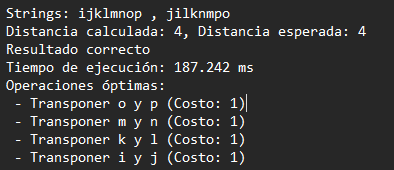
\includegraphics[width=0.45\textwidth]{images/trans-normal.png}
            \label{fig:imagen1}
        }
        \hfill
        % --
        \subfloat[Transposiciones con costo modificado.]{
            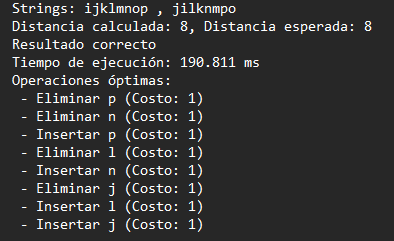
\includegraphics[width=0.45\textwidth]{images/trans-modificada.png}
            \label{fig:imagen2}
        }
        \caption{Ejemplo ejecución de transposiciones.}
        \label{fig:trans}
    \end{figure}

    Por lo tanto, al modificar los costos de las operaciones, no
    se modifica en gran medida el tiempo de ejecución de los algoritmos
    al igual con el uso de memoria, pero si las operaciones las cuales producen la distancia de edición
    minima. Por lo tanto,
    se evidencia que los costos de de las operaciones no afectan a la complejidad
    temporal y espacial.

    \item Cadenas vacías y caracteres repetidos
    
        \begin{table}[H]
        \centering
        \begin{tabular}{|c|c|c|}
        \hline
        \textbf{Tipo/Data} & \textbf{Cadenas vacías} & \textbf{Caracteres repetidos}\\ \hline
        Fuerza Bruta (ms) & 0.0033952 & 183.942 \\ \hline
        Programación Dinámica (ms) & 0.0099436 & 0.0952444 \\ \hline
        Memoria FB (KB) & 97.15 & 106.5   \\ \hline
        Memoria PD (KB) & 100.7 & 143.9 \\ \hline
      
        \end{tabular}
        \caption{Tabla con valores de prueba para cadenas vacías y caracteres repetidos}
        \label{tab:tabla2}
        \end{table}

    
    Para el dataset de cadenas vacías podemos observar que al algoritmo
    de fuerza bruta le toma menos tiempo en resolver la consulta con
    respecto al de programación dinámica. Por otro lado, el uso de memoria
    es similar en los dos casos.

    Estos resultados se deben a las complejidades temporales y espaciales
    de cada algoritmo, para el algoritmo de fuerza bruta, su tiempo de ejecución
    es exponencial con respecto al tamaño mas pequeño de la entrada, 
    al tener una entrada con largo 0, el algoritmo resuelve el problema
    muy eficientemente, podríamos decir que le toma tiempo $4^0=1$.

    Por el lado del algoritmo de programación dinámica, su tiempo de ejecución
    se modela según los tamaños de las dos entradas mas 1, por lo tanto, podríamos
    decir que le toma tiempo $1*9=9$, lo cual es mayor que el algoritmo de
    fuerza bruta.

    Ademas, los usos de memoria son similares ya que el algoritmo de 
    programación dinámica basa su uso de memoria en los tamaños de las
    dos entradas, al tener
    una de las entradas pequeñas, el uso de memoria disminuye.

    Sobre el dataset de caracteres repetidos, podemos observar que
    el algoritmo de fuerza bruta es mas ineficiente con respecto 
    al de programación dinámica, no obstante, el uso de memoria
    es mayor en este ultimo.

    Con esto, podemos evidenciar en la practica que las complejidades
    temporales y espaciales para cada algoritmo se cumplen.

    
    \item Palabras aleatorias con matrices de costo estándar y modificado
    
        \begin{table}[H]
        \centering
        \begin{tabular}{|c|c|c|c|c|}
        \hline
        \textbf{Data/Tipo} & \textbf{Fuerza Bruta (ms)} & \textbf{Programación Dinámica (ms)} & \textbf{Memoria FB (KB)} & \textbf{Memoria PD (KB)} \\ \hline
        Menor a 2 & 0.00890745 & 0.0101063 & 97.55 & 98.02\\ \hline
        3 a 4 & 0.15021 & 0.0225789 & 99.37 &  104 \\ \hline
        7 & 33.0569 & 0.0653561 & 105.2 & 131.1 \\ \hline
        8 & 180.548 & 0.0875144 & 108.2 & 145.6 \\ \hline
        8 Modificado & 181.627 & 0.0992815 & 105.5 & 145.2\\ \hline
        12 & 172570 & 0.219571 & No medido & 252.5\\ \hline
        \end{tabular}
        \caption{Tabla con valores de prueba para cadenas aleatorias}
        \label{tab:tabla3}
        \end{table}

    \begin{mdframed}
        El uso de memoria para las palabras de largo 12 con el algoritmo de 
        fuerza bruta no pudo ser medido ya que 
        se excedía el tiempo de ejecución con la utilidad \textbf{massif}.
    \end{mdframed}

    Para los datasets de palabras aleatorias podemos ver que nuevamente,
    el algoritmo de fuerza bruta es mas ineficiente frente al algoritmo
    de programación dinámica, exceptuando cuando la entrada es muy pequeña.
    Ademas podemos ver mas claramente el comportamiento a medida que crece el 
    tamaño de la entrada:


    \begin{figure}[H]
        \centering
      
        \subfloat[Tiempo de ejecución Fuerza Bruta.]{
            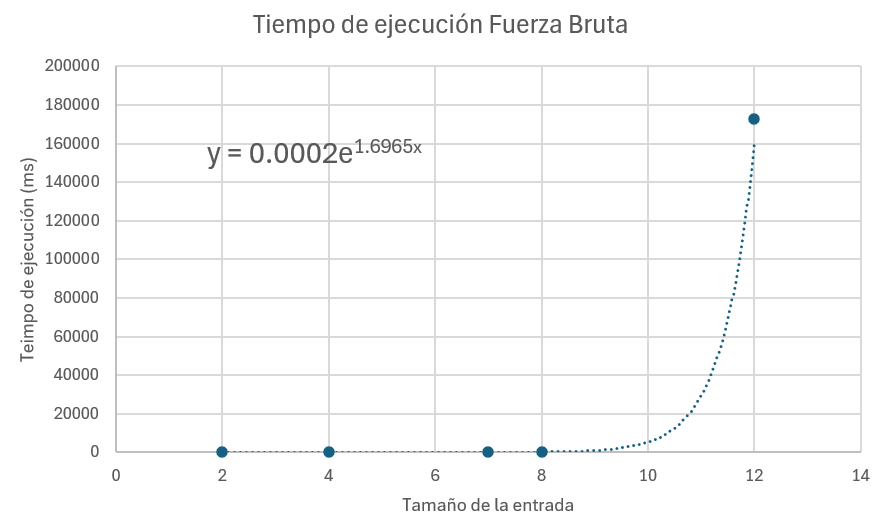
\includegraphics[width=0.5\textwidth]{images/tiempo-ejecucion-bf.png}
            \label{fig:imagen1}
        }
        % --
        \subfloat[Tiempo de ejecución Programación Dinámica.]{
            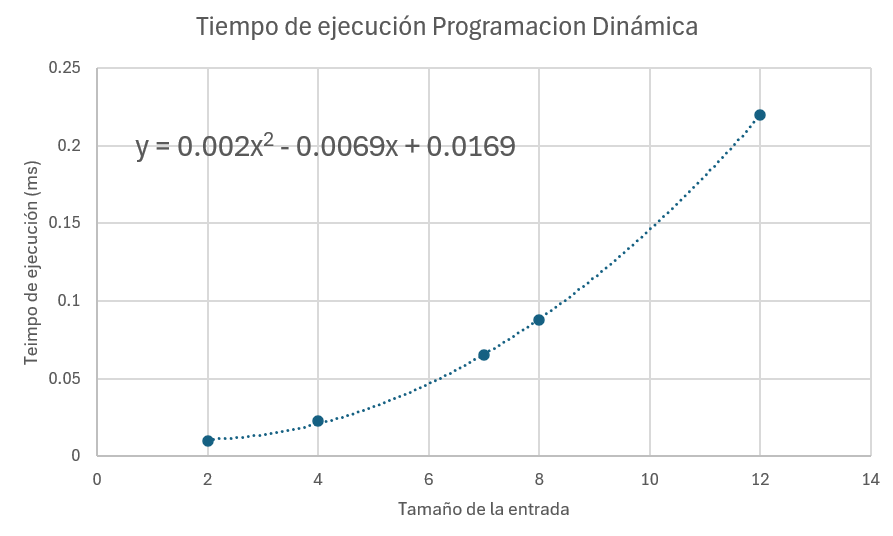
\includegraphics[width=0.5\textwidth]{images/tiempo-ejecucion-dp.png}
            \label{fig:imagen2}
        }

    \end{figure}

    \begin{figure}[H]
        \centering
      
        \subfloat[Uso de memoria Fuerza Bruta.]{
            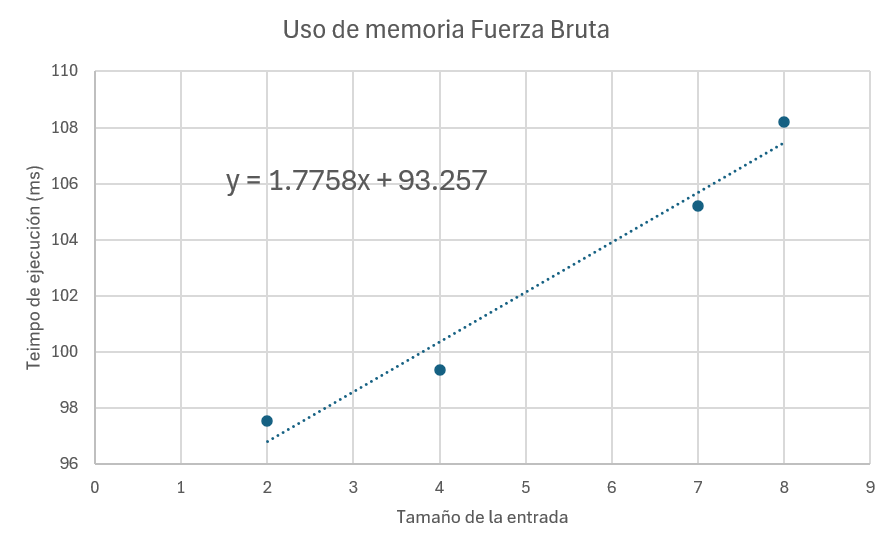
\includegraphics[width=0.5\textwidth]{images/usomem-bf.png}
            \label{fig:imagen1}
        }
        % --
        \subfloat[Uso de memoria Programación Dinámica.]{
            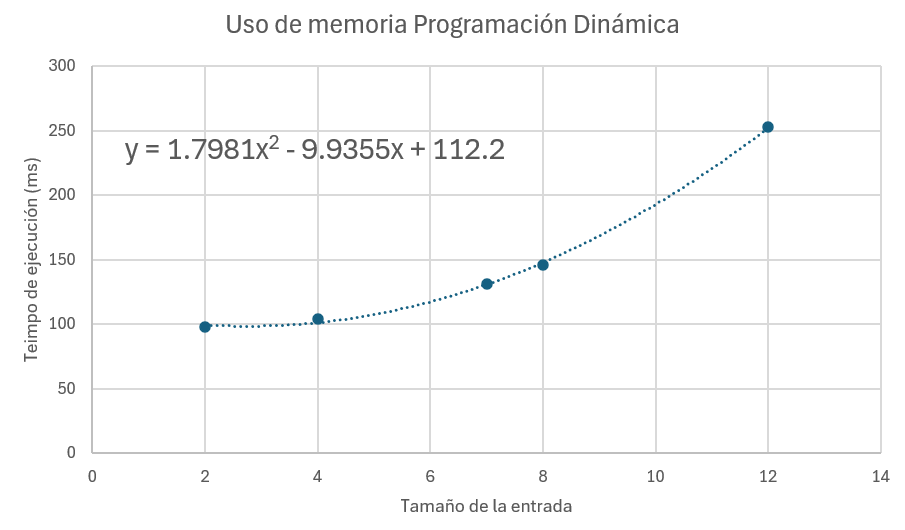
\includegraphics[width=0.5\textwidth]{images/usomem-dp.png}
            \label{fig:imagen2}
        }

    \end{figure}

    Los gráficos representan el tiempo de ejecución de los algoritmos
    a medida que crece la entrada, al igual que el uso de memoria, ademas
    se les agrego una linea de tendencia en conjunto con la ecuación del
    gráfico.

    Con esto, podemos determinar que a medida que crece la entrada,
    el tiempo de ejecución del algoritmo de fuerza bruta 
    se comporta de manera exponencial y su memoria se comporta
    de manera lineal.

    Por otra parte, el tiempo de ejecución del algoritmo de programación
    dinámica se comporta de manera cuadrática, al igual que su uso de 
    memoria.

    Ademas, con el dataset con costos modificados, no se observo mayores
    diferencias con respecto al resto de las pruebas, exceptuando la secuencia
    de operaciones que producen la distancia de edición optima, la cual
    cambio con respecto a las matrices de costo estándar.


\end{enumerate}















\begin{comment}


En esta sección, los resultados obtenidos, como las gráficas o tablas, deben estar respaldados por los datos generados durante la ejecución de sus programas. Es fundamental que, junto con el informe, se adjunten los archivos que contienen dichos datos para permitir su verificación. Además, se debe permitir y especficiar como obtener esos archivos desde una ejecución en otro computador (otra infraestructura para hacer lso experimentos).

\textbf{No es necesario automatizar la generación de las gráficas}, pero sí es imprescindible que se pueda confirmar que las visualizaciones presentadas son producto de los datos generados por sus algoritmos, aunque la trazabilidad de los datos hasta las visualizaciones es esencial para garantizar que su validez: describa cómo se generaron los datos, cómo se procesaron y cómo se visualizaron de manera que pueda ser replicado por quien lea su informe.

Agregue gráficas que muestren los resultados de sus experimentos. La cantidad de páginas es limitada, por lo tanto escoja las gráficas más representativas y que muestren de manera clara los resultados obtenidos. Esta elección es parte de lo que se evaluara en la sección de presentación de resultados. Referencie las figuras en el texto, describa lo que se observa en ellas y por qué son relevantes.

En la \cref{fig:scatterplot_1} se muestra un scatterplot hecho con \href{https://es.overleaf.com/learn/latex/TikZ_package}{TikZ} con el tamaño ideal cuando se incluyen dos figuras. Queda a criterio de usted el decidir qué figuras incluir.

\begin{figure}[H]
    \centering
    
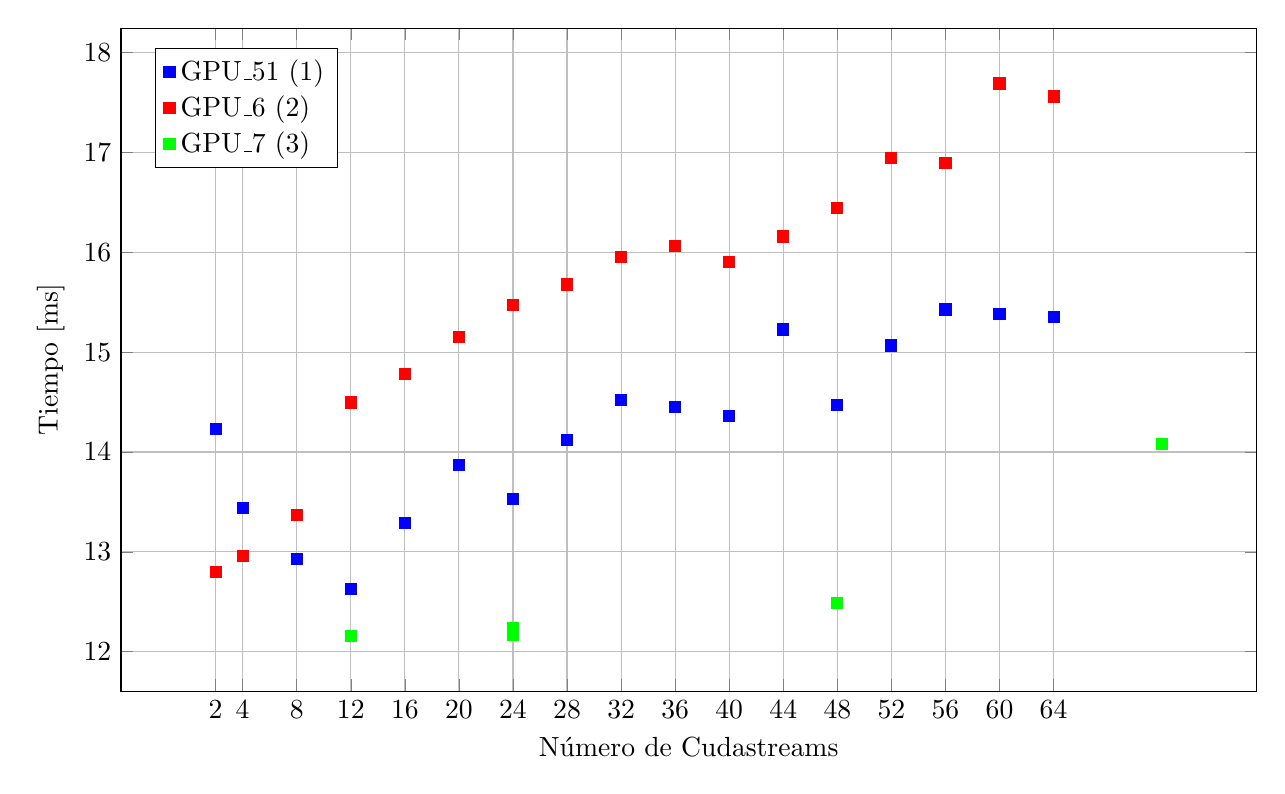
\begin{tikzpicture}
    %\begin{loglogaxis}[
    %\begin{semilogxaxis}[ % Cambiar a semilogxaxis    
    \begin{axis}[
        xlabel={Número de Cudastreams },
        ylabel={Tiempo [ms]},
        grid=major,
        legend pos=north west,
        legend cell align={left},
        width=16cm,
        height=10cm, 
        xtick=data,
    ]
    \addplot[blue, only marks, mark=square*] coordinates {
        (2   , 14.229344)
        (4   , 13.435616 )
        (8   , 12.929280 )
        (12  , 12.628000 )
        (16  , 13.286176 )
        (20  , 13.873152 )
        (24  , 13.531168 )
        (28  , 14.116384 )
        (32  , 14.518528 )
        (36  , 14.448992 )
        (40  , 14.356640 )
        (44  , 15.226560 )
        (48  , 14.473888 )
        (52  , 15.066720 )
        (56  , 15.426560 )
        (60  , 15.380416 )
        (64  , 15.348064 )
    };
    \addlegendentry{GPU\_51 (1)}
    \addplot[red, only marks, mark=square*] coordinates {
        (2  , 12.799264 ) 
        (4  , 12.956192 )
        (8  , 13.371104 )
        (12 , 14.495616 )
        (16 , 14.783360 ) 
        (20 , 15.152672 ) 
        (24 , 15.475488 ) 
        (28 , 15.676416 ) 
        (32 , 15.948800 ) 
        (36 , 16.064129 ) 
        (40 , 15.904544 ) 
        (44 , 16.157921 ) 
        (48 , 16.444992 ) 
        (52 , 16.943169 ) 
        (56 , 16.894304 ) 
        (60 , 17.689600 ) 
        (64 , 17.559551 ) 
    };
    \addlegendentry{GPU\_6 (2)}
    \addplot[green, only marks, mark=square*] coordinates {
        (6, 17.607168) 
        (12, 12.159264) 
        (24, 12.239648) 
        (24, 12.169376) 
        (48, 12.490624) 
        (72, 14.081920) 
    };
    \addlegendentry{GPU\_7 (3)}
   
\end{axis}
%\end{semilogxaxis} % Cambiar a semilogxaxis
\end{tikzpicture}

    \caption{Ejemplo de scatterplot hecho con tikz. Tamaño ideal 1.}
    \label{fig:scatterplot_1}
\end{figure}


\begin{figure}[H]
    \centering
    \begin{minipage}[t]{0.5\textwidth}
    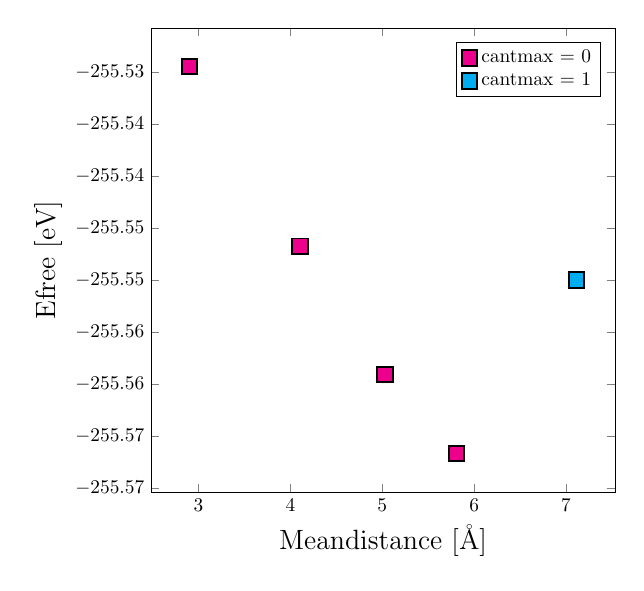
\begin{tikzpicture}[scale=0.7]
    %\begin{loglogaxis}[
    %\begin{semilogxaxis}[ % Cambiar a semilogxaxis    
    \begin{axis}[
        xlabel={\Large Meandistance [\AA] },
        ylabel={\Large Efree [eV]},
        %grid=major,
        legend pos=north east,
        legend cell align={left},
        %log basis x=10,
        %log basis y=10,
        %xmin=2, xmax=2^21,
        %ymin=0.1, ymax=100,
        width=10cm, % Ajusta el ancho de la gráfica
        height=10cm, % Ajusta la altura de la gráfica
        %xtick=data,
    ]
    \addplot[magenta , only marks, mark=square*, mark options={draw=black,line width = 1pt}, mark size=4pt] coordinates {
        %(7.112914 ,	-255.554964)
        (5.807670 ,	-255.571675)
        (2.903835 ,	-255.534455)
        (5.029590 ,	-255.564079)
        (4.106643 ,	-255.551738)       
        };
    \addlegendentry{cantmax = 0} 
    \addplot[cyan , only marks, mark=square*, mark options={draw=black,line width = 1pt}, mark size=4pt] coordinates {
        (7.112914 ,	-255.554964)   
        };
        \addlegendentry{cantmax = 1} 
\end{axis}
%\end{semilogxaxis} % Cambiar a semilogxaxis
\end{tikzpicture}
    \end{minipage}%
    \begin{minipage}[t]{0.5\textwidth}
    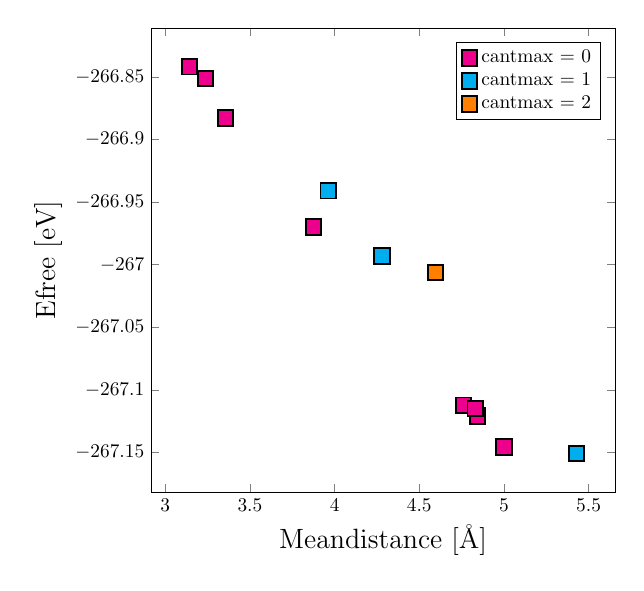
\begin{tikzpicture}[scale=0.7]
    %\begin{loglogaxis}[
    %\begin{semilogxaxis}[ % Cambiar a semilogxaxis    
    \begin{axis}[
        xlabel={\Large Meandistance [\AA] },
        ylabel={\Large Efree [eV]},
        %grid=major,
        legend pos=north east,
        legend cell align={left},
        %log basis x=10,
        %log basis y=10,
        %xmin=2, xmax=2^21,
        %ymin=0.1, ymax=100,
        width=10cm, % Ajusta el ancho de la gráfica
        height=10cm, % Ajusta la altura de la gráfica
        %xtick=data,
    ]
    \addplot[magenta , only marks, mark=square*, mark options={draw=black,line width = 1pt}, mark size=4pt] coordinates {
        (4.845001   ,	-267.121023)	% 0
        (5.000617   ,	-267.145714)	% 0
        (4.760055   ,	-267.112360)	% 0
        (3.236691   ,	-266.851158)	% 0
        (3.356972   ,	-266.882713)	% 0
        %(5.427886   ,	-267.150822)	% 1
        (4.830514   ,	-267.115114)	% 0
        (3.144397   ,	-266.841800)	% 0
        %(4.280839   ,	-266.992946)	% 1
        (3.874418   ,	-266.969850)	% 0
        %(4.595953   ,	-267.006159)	% 2
        %(3.962469   ,	-266.940902)	% 1       
        };
    \addlegendentry{cantmax = 0} 
    \addplot[cyan , only marks, mark=square*, mark options={draw=black,line width = 1pt}, mark size=4pt] coordinates {
        (5.427886   ,	-267.150822)	% 1
        (4.280839   ,	-266.992946)	% 1
        (3.962469   ,	-266.940902)	% 1
        };
        \addlegendentry{cantmax = 1} 
    \addplot[orange , only marks, mark=square*, mark options={draw=black,line width = 1pt}, mark size=4pt] coordinates {
        (4.595953   ,	-267.006159)	% 2
        };
        \addlegendentry{cantmax = 2}
\end{axis}
%\end{semilogxaxis} % Cambiar a semilogxaxis
\end{tikzpicture}
    \end{minipage}%
    \caption{Ejemplo de scatterplot hecho con tikz. Tamaño ideal 2.}
    \label{fig:scatterplot_2}
\end{figure}

\begin{figure}[H]
    \centering
    \begin{minipage}[t]{0.5\textwidth}
        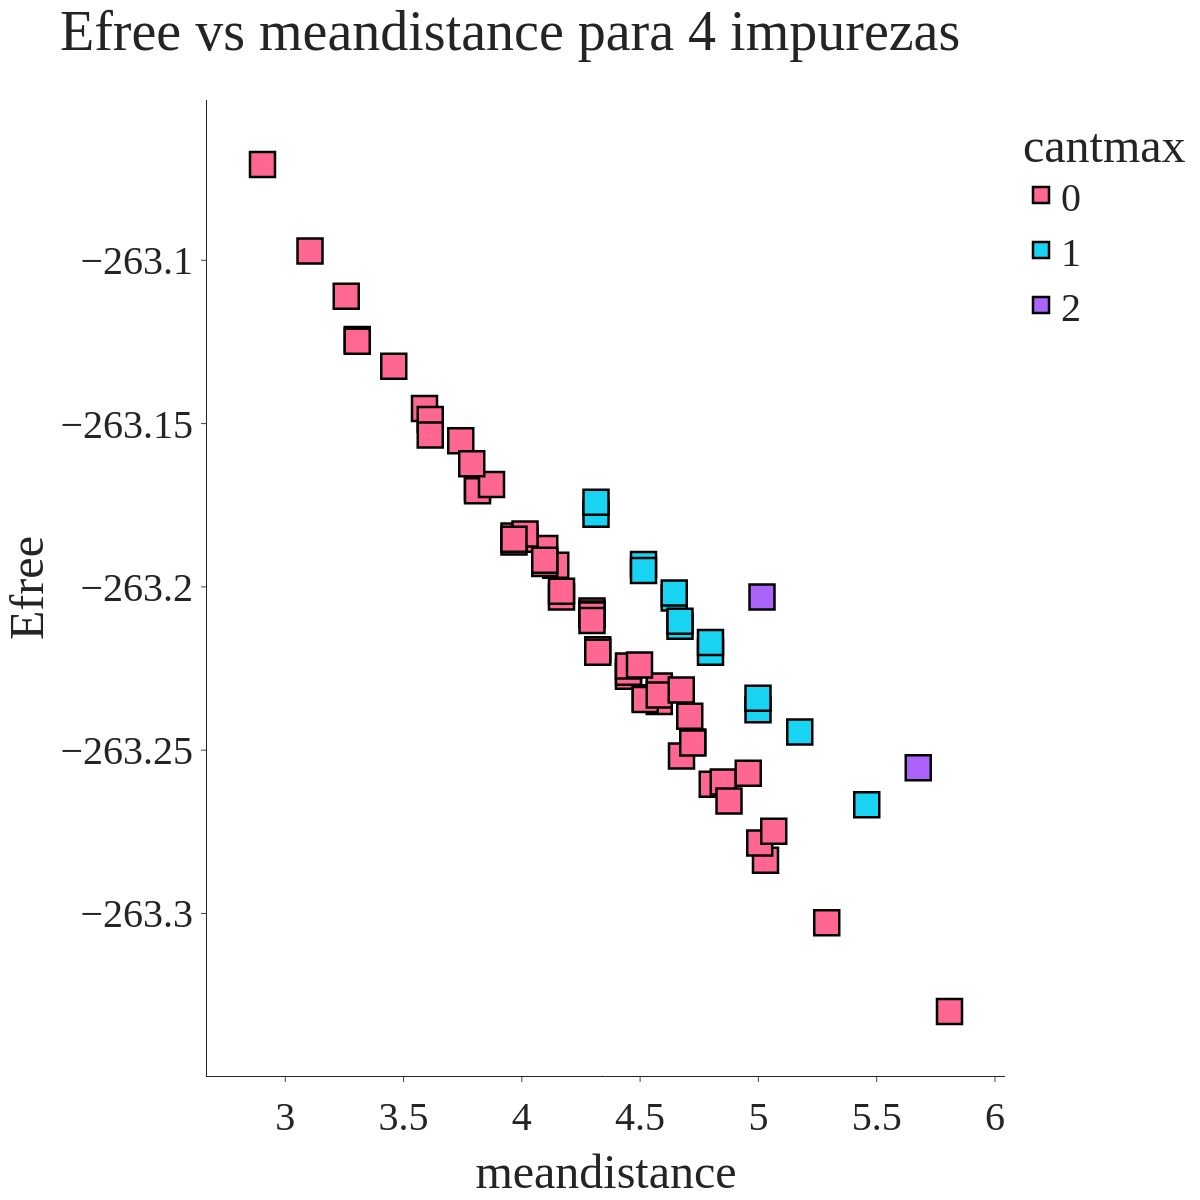
\includegraphics[width=\textwidth]{images/4_impurezas_cantmax_size10.png}
    \end{minipage}%
    \begin{minipage}[t]{0.5\textwidth}
        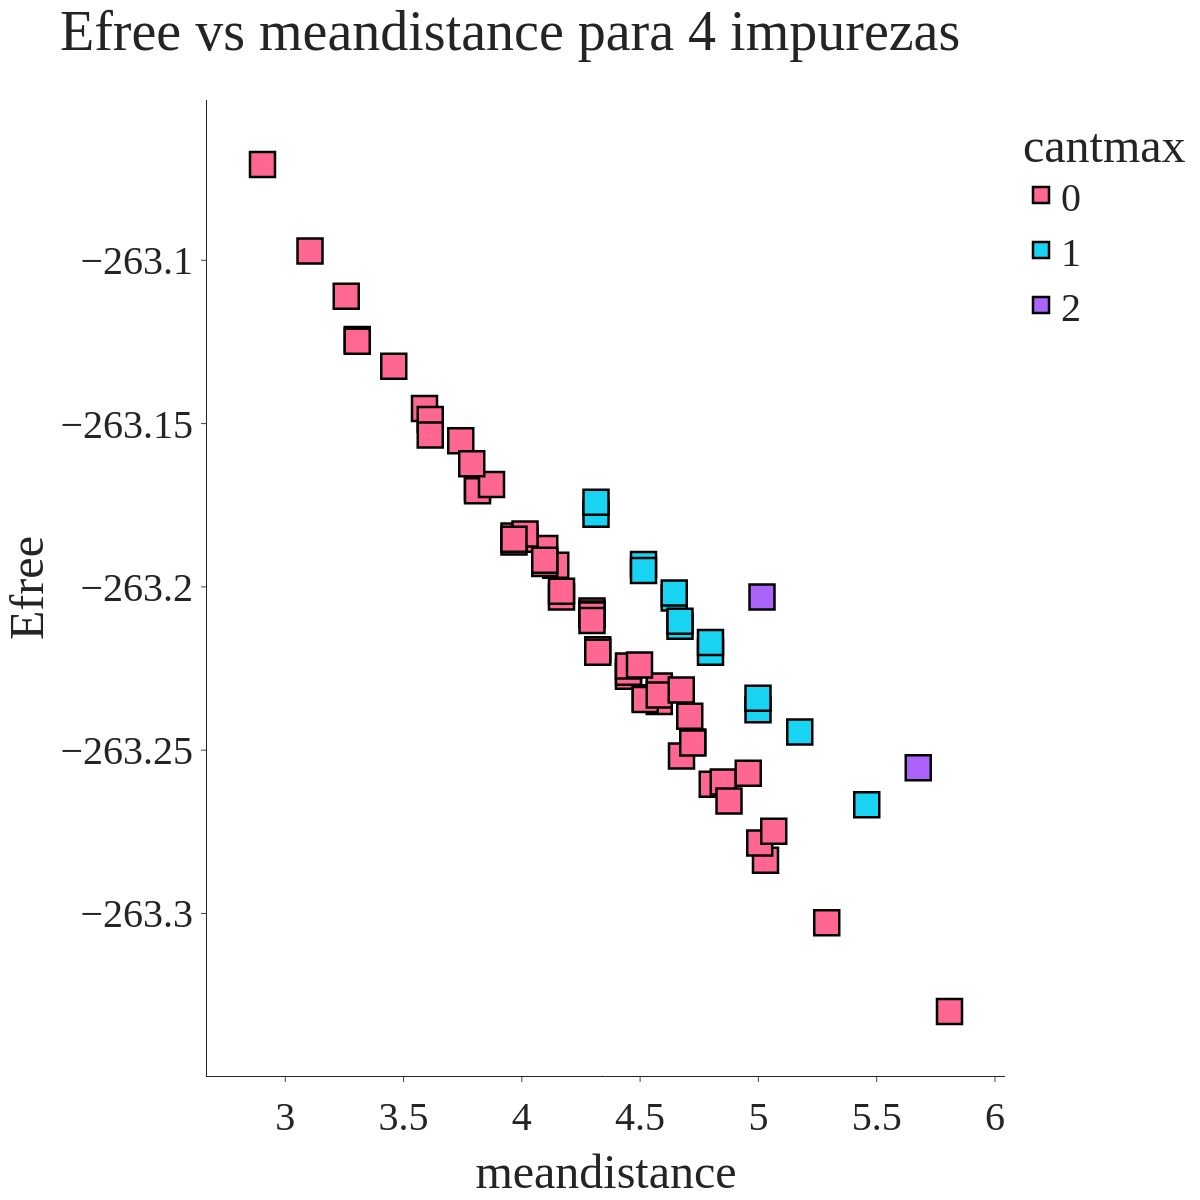
\includegraphics[width=\textwidth]{images/4_impurezas_cantmax_size10.png}    \end{minipage}%
    \caption{Ejemplo de scatterplot hecho con matplotlib.}
    \label{fig:scatterplot_3}
\end{figure}



\begin{mdframed}
    Recuerde que es imprescindible que se pueda replicar la generación de las gráficas, por lo que usted debe incluir cómo generó esos datos y  cómo podría generarlos la persona que revisa su entrega y ejecuta sus programas. Por ejemplo, si genera un scatterpolot con Tikz, usted debe explicar cómo obtener la tupla de valores que se usaron para generar la gráfica.
\end{mdframed}

\end{comment}